\documentclass[tikz,border=1.35mm]{standalone}

\definecolor{fvmadaptedge}{HTML}{8A7E7E}
\usetikzlibrary{arrows.meta}

\definecolor{externalface}{HTML}{8FB9E8}

% Irregular eight-faced polyhedral cell.
% This is a skewed brick with two opposite corners clipped away. The result has
% triangular and pentagonal faces, which makes it read as a generic polyhedron
% rather than one of the named cell types.
\begin{document}
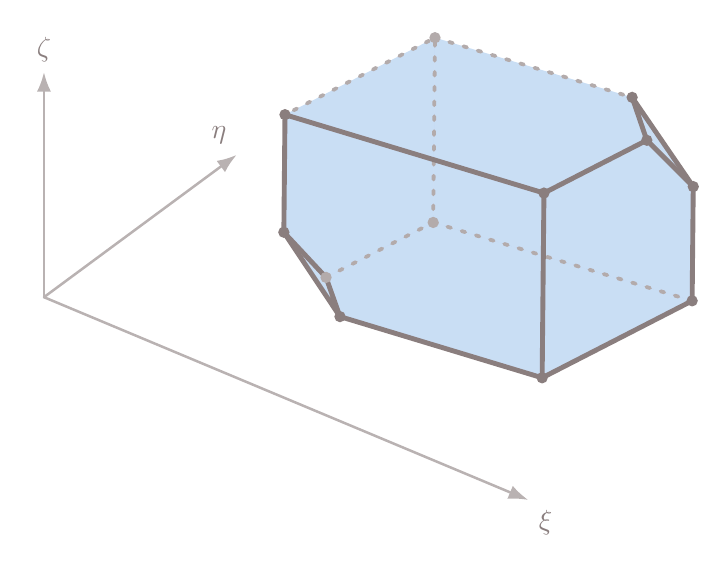
\begin{tikzpicture}[
  x={(20.3mm,-8.5mm)},
  y={(15.3mm,11.3mm)},
  z={(0mm,20mm)},
  line join=round,
  line cap=round,
  outer/.style={draw=fvmadaptedge,line width=0.62mm},
  hidden/.style={draw=fvmadaptedge!65,line width=0.48mm,loosely dotted},
  face/.style={fill=externalface,fill opacity=0.28,draw=none},
  axis/.style={draw=fvmadaptedge!60,line width=0.32mm,-{Latex[length=2.5mm,width=1.8mm]}}
]
  % The coordinates come from an affine-skewed brick with the xi/eta/zeta-min
  % and xi/eta/zeta-max corners clipped. The affine skew keeps faces planar
  % while avoiding a too-regular box-like appearance.
  \coordinate (Oxi) at (0.3400,0.0204,0.0238);
  \coordinate (Oeta) at (0.0420,0.3000,-0.0120);
  \coordinate (Ozeta) at (-0.0200,0.0320,0.4000);
  \coordinate (B) at (1.5500,0.0930,0.1085);
  \coordinate (C) at (1.6970,1.1430,0.0665);
  \coordinate (D) at (0.1470,1.0500,-0.0420);
  \coordinate (E) at (-0.0550,0.0880,1.1000);
  \coordinate (F) at (1.4950,0.1810,1.2085);
  \coordinate (H) at (0.0920,1.1380,1.0580);
  \coordinate (Gxi) at (1.2720,1.2088,1.1406);
  \coordinate (Geta) at (1.5958,0.9010,1.1797);
  \coordinate (Gzeta) at (1.6630,1.1974,0.7465);

  % Offset computational-coordinate axes.
  \coordinate (Oaxis) at (-1.18,-0.42,-0.25);
  \draw[axis] (Oaxis) -- (1.85,-0.42,-0.25) node[below right,font=\normalsize,text=fvmadaptedge] {$\xi$};
  \draw[axis] (Oaxis) -- (-1.18,1.18,-0.25) node[above left,font=\normalsize,text=fvmadaptedge] {$\eta$};
  \draw[axis] (Oaxis) -- (-1.18,-0.42,1.18) node[above,font=\normalsize,text=fvmadaptedge] {$\zeta$};

  % Exterior faces share one translucent shade. Faces are drawn back-to-front by
  % hand so the visible edges remain readable.
  \path[face] (Oeta) -- (D) -- (H) -- (E) -- (Ozeta) -- cycle;
  \path[face] (D) -- (C) -- (Gzeta) -- (Gxi) -- (H) -- cycle;
  \path[face] (E) -- (F) -- (Geta) -- (Gxi) -- (H) -- cycle;
  \path[face] (Gxi) -- (Geta) -- (Gzeta) -- cycle;
  \path[face] (Oxi) -- (B) -- (C) -- (D) -- (Oeta) -- cycle;
  \path[face] (Oxi) -- (B) -- (F) -- (E) -- (Ozeta) -- cycle;
  \path[face] (B) -- (C) -- (Gzeta) -- (Geta) -- (F) -- cycle;
  \path[face] (Oxi) -- (Oeta) -- (Ozeta) -- cycle;

  % A few far-side edges are dotted to avoid making the transparent cell look
  % like all edges are equally close to the viewer.
  \draw[hidden] (Oeta) -- (D) -- (H) -- (E);
  \draw[hidden] (D) -- (C);
  \draw[hidden] (H) -- (Gxi);

  % Visible exterior wireframe.
  \draw[outer] (Oxi) -- (B) -- (C) -- (Gzeta) -- (Geta) -- (F) -- (B);
  \draw[outer] (E) -- (F);
  \draw[outer] (E) -- (Ozeta) -- (Oxi) -- (Oeta);
  \draw[outer] (Oeta) -- (Ozeta);
  \draw[outer] (Geta) -- (Gxi) -- (Gzeta);

  % Original vertices are #8a7e7e, with far-side vertices softened.
  \foreach \p in {Oxi,Ozeta,B,C,E,F,Gxi,Geta,Gzeta} {
    \fill[fvmadaptedge] (\p) circle[radius=0.72mm];
  }
  \foreach \p in {Oeta,D,H} {
    \fill[fvmadaptedge!65] (\p) circle[radius=0.72mm];
  }
\end{tikzpicture}
\end{document}
